\documentclass{beamer}

\usepackage{graphicx}
\usepackage{subcaption}

\usepackage{amsmath}
\usepackage{algorithm}
\usepackage{algpseudocode}

\graphicspath{ {images/} }

\usetheme{Madrid}
\usecolortheme{beaver}

\title{Inference in Wargame}
\author{Zhuo Yueyi}
\institute[NUST]{}
\date{17/10/2019}

\begin{document}

\frame{\titlepage}

\begin{frame}

For gameplay or simplicity. Wargame and strategy game tend to give full information about its model.

\begin{figure}[htb]
    \centering
    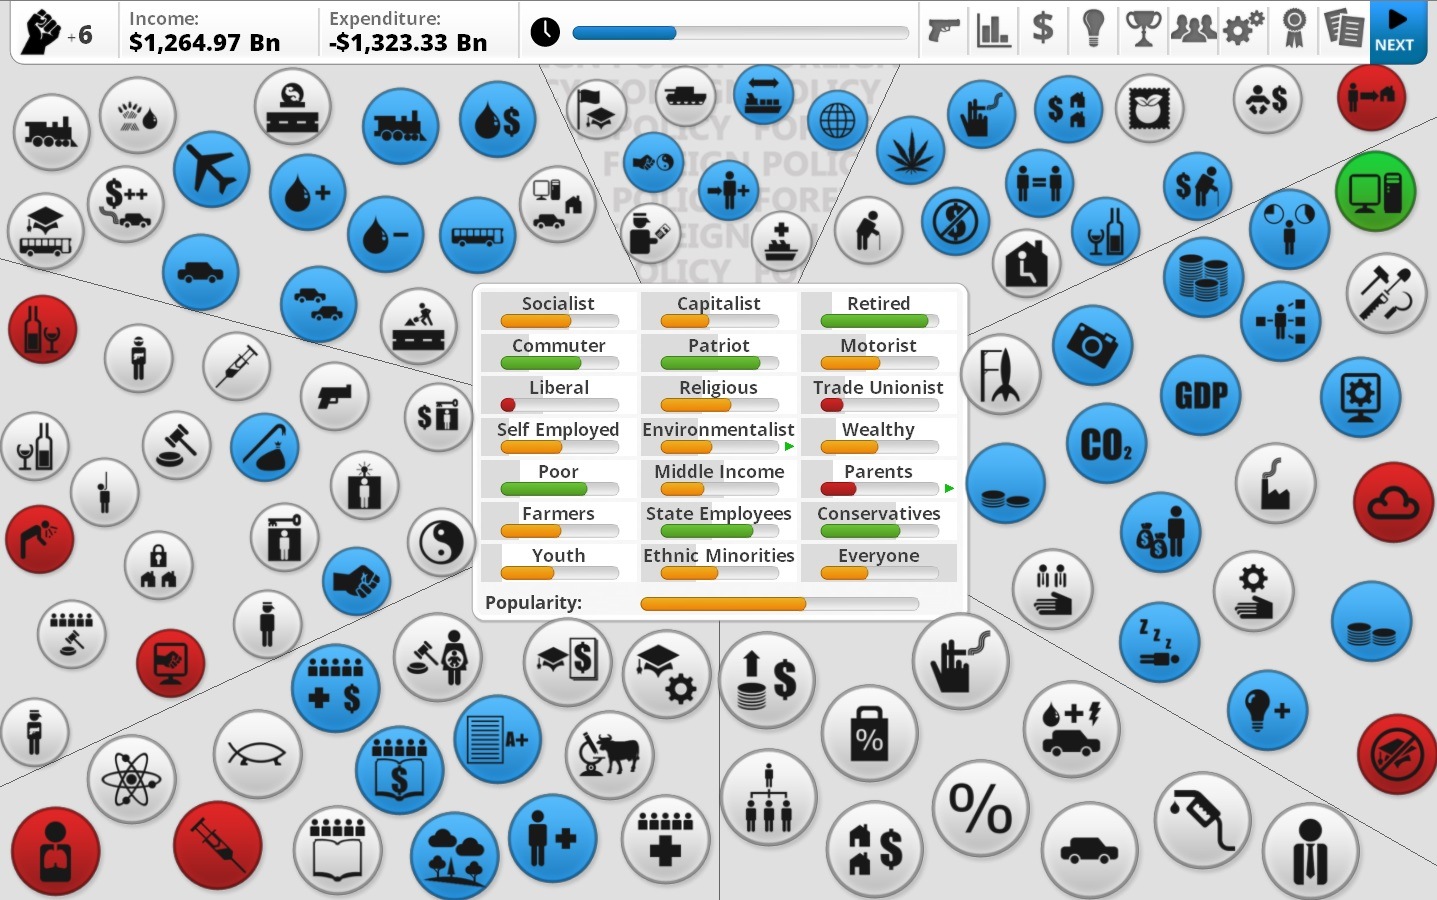
\includegraphics[width=0.7\linewidth]{dd3.jpg}
    \caption{A Screenshot of Democracy 3}
\end{figure}

A nice and brief sketch to present leader such as Trump or Sager King(?)

\end{frame}

\begin{frame}

\frametitle{Mao's legacy}

    \begin{figure}[htb]
        \centering
        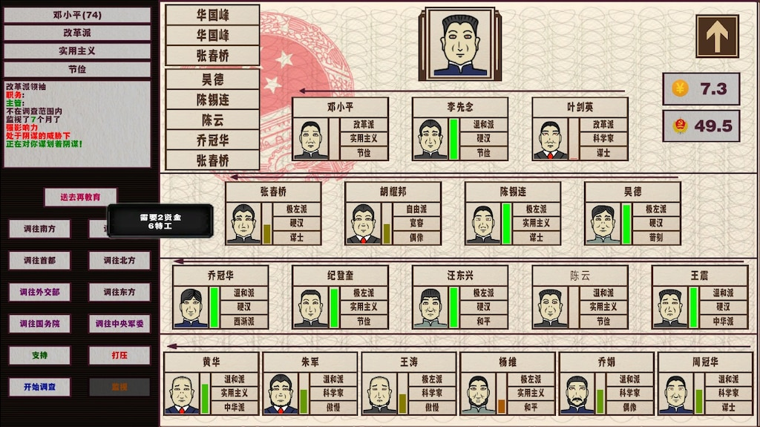
\includegraphics[width=0.7\linewidth]{mao_legacy.png}
    \end{figure}    

\begin{itemize}

\item Hua GuoFeng, controlled by player, is trying to capture Deng using 2 money and 6 agent.

\item Why can you see attitude of those conspirators directly. It seems that they're all sheep waiting your slaughter! 

\end{itemize}

\end{frame}

\begin{frame}

\frametitle{Case Study: Heart of Iron IV }

\begin{columns}[T]
    \begin{column}{.5\textwidth}
        % Your image included here
            
\includegraphics[width=\textwidth]{hoi4.jpg}
    \end{column}        
    \begin{column}{.5\textwidth}
% Your text here

\begin{itemize}
\item Italian General, Giovanni Messe, commanding 4 Italian divisions attack 2 Ethiopia divisions in Second Italo-Ethiopian War. 

\item It may be great to see a such detailed summary without any error to a ideal dictator. But how about hiding some related information?
\end{itemize}

    \end{column}
\end{columns}

\end{frame}

\begin{frame}

    \frametitle{Maybe a more realistic decision UI }
    
    \begin{columns}[T]
        \begin{column}{.5\textwidth}
            % Your image included here
                
\includegraphics[width=\textwidth]{hoi4_hidden.jpg}
        \end{column}        
        \begin{column}{.5\textwidth}
    % Your text here

    \begin{itemize}

    \item General Giovanni Messe:
    I can't figure out the situation at all! Should I retreat to avoid a decisive failure happened in  Battle of Adwa
    \item Battle of Adwa:
    In First Italo-Ethiopian War, 17700 Italians is defeated by 80000 Ethiopian soldiers in Adwa. This failure lead to a shameful peaceful treaty to Italian.

    \end{itemize}
    
    \end{column}
\end{columns}
    
\end{frame}
    
\begin{frame}
    \frametitle{Land Combat Resolution of HOI4}

    \begin{itemize}
    
    \item Every hour resolve a combat. 

    \item Every activated unit select a target randomly. 

    \item Comparing soft/hard attack value of attacker with  hardness, breakthrough and defense of defender, 
    attacker, some hits are determined with 60\% or 90\% probability.

    \item For each hit, rolling 2/4 dices for HP and organization.
    Target take corresponding damage to HP and organization modified by current strength of attacker.
    \end{itemize}
    
\end{frame}

\begin{frame}
    \frametitle{A simplified one turn model}
    % prior distribution of Attack-X, defense-X are ignored for simplicity.

    \begin{columns}[T]
        \begin{column}{.6\textwidth}
            $$
            \begin{aligned}
            i &\in 1,\dots,L \\
            j &\in 1,\dots, N \\
            N &\sim Possion(\lambda) \\
            TargetA_{i} &\sim Cat(1/N \,\mathbf{1})  \\
            TargetD_{j} &\sim Cat(1/L \, \mathbf{1})  \\
            HitA_i &\sim f(AttackA(i), DefenseD(TargetA_i)) \\
            HitD_j &\sim f(AttackD(j), DefenseA(TargetD_j)) \\
            LossHPA_i &\sim g(HitA_i, HPA(i)) \\
            LossHPD_j &\sim g(HitD_j, HPD(j))
            \end{aligned}
            $$
    \end{column}        
    \begin{column}{.4\textwidth}

        \begin{itemize}
        \item i,j are indexes of attacker and defender. 

        \item Attack-X denote soft and hard attack. Defense-X include defense, break through and hardness.
        \end{itemize}
                
    \end{column}
\end{columns}

\end{frame}

%\begin{frame}
%\frametitle{Challenge: Too many latent variables}
%\end{frame}
\begin{frame}

    \frametitle{Quaker gun}

        \begin{figure}[htb]
            \centering
            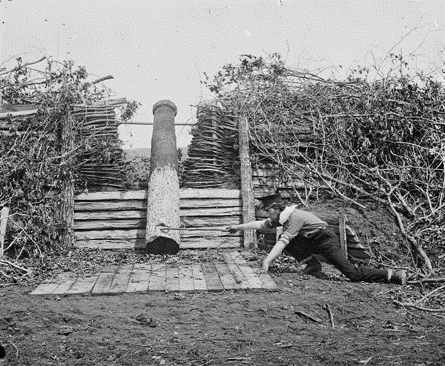
\includegraphics[width=0.4\linewidth]{quake_gun.png}
        \end{figure}    
    
        \begin{itemize}
        \item Quaker gun near Centreville, Virginia, in March 1862, after the Confederate withdrawal; a man with a stick is pretending to "fire" it with a linstock.
        \item General McClellan, confused by those sticks few months and reject to attack air.
        \end{itemize}

\end{frame}

\begin{frame}
    \frametitle{Related work: Starcraft Enemy Unit Count Inference}

    \begin{figure}[htb]
        \centering
        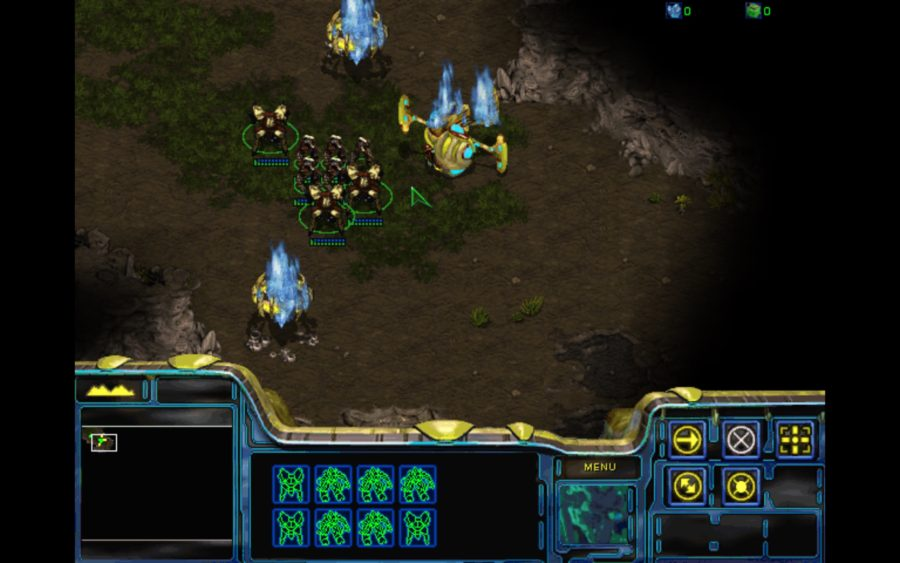
\includegraphics[width=0.7\linewidth]{starcraft.jpg}
    \end{figure}

    A model \footnote{Hostetler, Jesse, et al. "Inferring strategies from limited reconnaissance in real-time strategy games." Proceedings of the Twenty-Eighth Conference on Uncertainty in Artificial Intelligence. AUAI Press, 2012.
    } infer hidden enemy unit state using incomplete scouting.

\end{frame}

\begin{frame}
    \frametitle{Model specification}

    The model is given by a dynamic bayesian network, the two slicing plate notation graph is shown below:

    \begin{columns}[T]

    \begin{column}{.4\textwidth}
    \begin{figure}[htb]
        \centering
        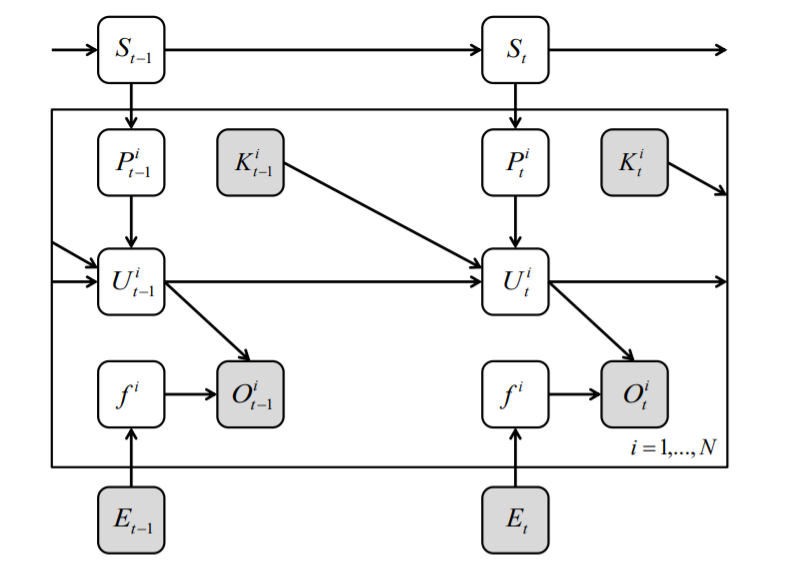
\includegraphics[width=0.9\linewidth]{starcraft_pg.png}
    \end{figure}    

    \end{column}
    \begin{column}{.6\textwidth}
        \begin{itemize}
            \item $S$: Hidden strategy state.
            \item $P^i$: Produced type $i$ unit.
            \item $K^i$: Killed type $i$ unit.
            \item $U^i$: Current type $i$ unit.
            \item $O^i$: Observed type $i$ unit.
            \item $f^i$: A middle variable determined by $E$.
            \item $E$: Effort of scouting.
        \end{itemize}
    \end{column}

    \end{columns}

    Gray node is observed variable, white node is latent variable. 
    The box(plate) mean independence given extern variables.

\end{frame}

\begin{frame}

Strategy model, a standard markov process:

\begin{align*}
P(S_0) &\sim Multinomial(\eta_1,\dots,\eta_M) \\
P(S_t|S_{t-1} = s) &= Multinomial(\pi_1^s,\dots,\pi_M^s)
\end{align*}

Production model:

$$
P(P_t^i = k|S_t=s)=\begin{cases}
    1 - \nu_s^i & k=0 \\
    \nu_s^i \dot Pois(k-1;\lambda_s^i) & k>0
\end{cases}
$$

Unexpected loss model:

\begin{align*}
    U_0^i &= c^i \\
    U_t^i &\sim Binomial(U_{t-1}^i - K_{t-1}^i, 1-l^i) + P_t^i
\end{align*}

Observation model:

\begin{align*}
    O_t^i &\sim BetaBinomial(U_t^i,\mu_t^i,\rho^i) \\
    \mu, \rho &= f_\theta(E_t)
\end{align*}    

\end{frame}

\begin{frame}
    \frametitle{Learning}

    \begin{itemize}

    \item Parameters include $\mathbf{\eta}, \mathbf{\pi}, \mathbf{\nu}, \mathbf{l}, \mathbf{\theta}$ .
    \item Since $P$ is observed in training, usual learning method for HMM such as EM algorithm
     can be employed to estimate $\mathbf{\eta}, \mathbf{\pi}$.
    \item Since $U$ is observed in training, we can fit $\mathbf{\theta}$ using any optimizing method with MLE can be used.
    \item denoting unobserved loss probability, denoted by $\mathbf{l}$, can be fitted using basic mean, given $U,f$.
    \item Those parameters are fixed in following inference.
    \end{itemize}
\end{frame}

\begin{frame}
    \frametitle{Inference: Particle Filtering}

    \begin{itemize}
        \item Kalman filtering assume Normal prior and linear transition, while Particle Filtering relax those requirements.
        \item Importance sampling: Given proposal distribution $q(x)$ $E_p(f(x)) = E_q(f(x)p(x)/q(x))$. 
        \item In general, a $q(x)$ more close to $p(x)$ will be preferred. 
        \item In PF
            \footnote{Doucet, Arnaud, et al. "Rao-Blackwellised particle filtering for dynamic Bayesian networks." Proceedings of the Sixteenth conference on Uncertainty in artificial intelligence. Morgan Kaufmann Publishers Inc., 2000.},
            posterior probability $P(S_t|Y_{1:t})$ is approximated by R "particles" $S_t^r$ with weight $w_t^r$, giving a discrete probability: $\bar{P}(S_t = s_t|Y_{1:t}) = \sum_{r=1}^R w_t^r I(S_t = s_t)$
        \item From $\bar{P}(S_t = s_t|Y_{1:t-1})$, R new particles are drawn using $Q(S_t) = P(S_t|s_{t-1})$. 
        \item Following importance sampling, Weight will be given by:
    \end{itemize}
\end{frame}

\begin{frame}
    \frametitle{Particle Filtering: Weight update}

    \begin{align*}
        w_0^r &= (P(y_0|s_r)P(s_r))/Q(s_r) \\
        w_t^r &= w_{t-1}^r w_t^{r'} \\
        w_t^{r'} &= \frac{P(Y_t = y_t|y_{0:t-1}, s_{0:t}^r)P(S_t=s_t^r|S_{t-1}=s_{t-1}^r)}{P(S_t=s_t^r|S_{t-1}=s_{t-1}^r)} \\
            &= P(Y_t=y_t|y_{0:t-1},s_{0:t}^r) \\
            &= \prod_{i=1}^N P(U_t^i|U_{t-1}^i,P_t^i,K_{t-1}^i)P(U_{t-1}^{i,r}) P(P_t^i|S_t=s_t^r)P(O_t^i|U_t^i,E_t^i)
    \end{align*}

    \begin{itemize}
        \item $Y_t$ is collection of observed variable: $Y_t = \{ \mathbf{E}, \mathbf{K}, \mathbf{O} \} $.
    \end{itemize}

\end{frame}

\begin{frame}
    \frametitle{Performance: Unit Counting}

    \begin{columns}[T]

    \begin{column}{.5\textwidth}

    \begin{figure}[htb]
        \centering
        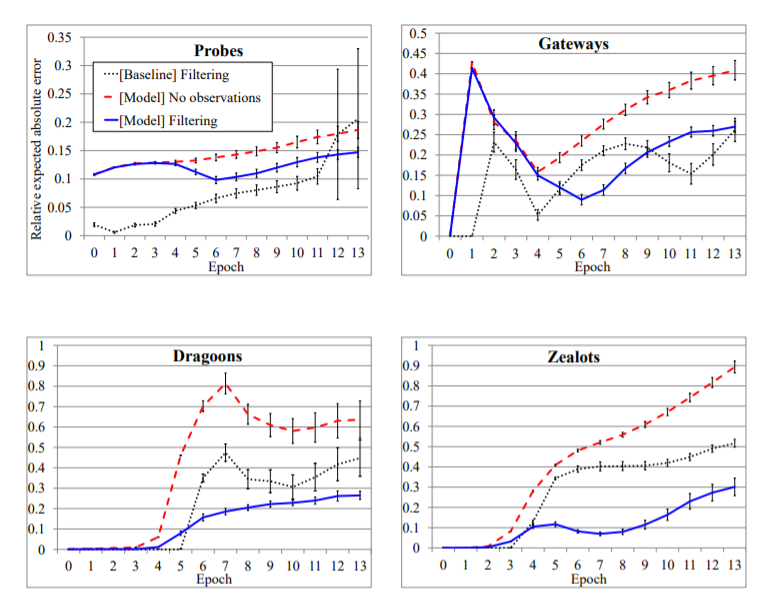
\includegraphics[width=0.95\linewidth]{sc1.png}
    \end{figure}

    \end{column}

    \begin{column}{.5\textwidth}

        \begin{figure}[htb]
            \centering
            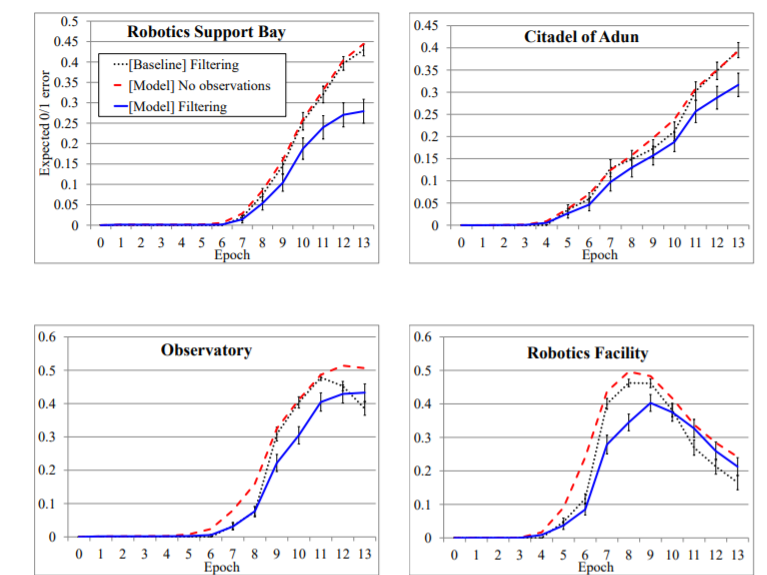
\includegraphics[width=0.95\linewidth]{sc2.png}
        \end{figure} 
        
    \end{column}

    \end{columns}

    Relative expected absolute error is given by:
    $$
    \epsilon_t^i = E(|U_t^i - u_t^i|)/(u_t^i+1)
    $$

\end{frame}


%\begin{frame}
%    \frametitle{Particle Gibbs}
%\end{frame}

\begin{frame}
    \frametitle{Observing Local: Laplace approximation}

    Leveraging special structure of integral, high dimensional integral can be approximated by
    Gauss Hermite quadrature:
    $$
    \int_{-\infty}^{\infty} e^{-x^2}f(x)dx \approx \sum_{i=1}^n w_i f(x_i)
    $$

    While cost of GMQ is not proportional to domain of $f$, it still suffer from curse of dimension.
    Thus, Laplace approximation for integral is considered:
    $$
    \int_a^b e^{Mf(x)}dx \approx \sqrt{\frac{2\pi}{M|f''(x_0)|}}e^{Mf(x_0)}
    $$

    The complexity is $d^2$ instead of $n^d$ in GMQ. 

\end{frame}

\begin{frame}

    Adding some extra approximation, tt lead to a result just like asymptotic property MLE:

    $$
    p(\theta|x) \approx N(\hat{\theta}, I(\hat{\theta})^{-1})
    $$

    Where $\hat{\theta}$ is MAP, and $I(\theta)$ is observed fisher information:

    $$
    I(\theta) = -\frac{d^2}{d\theta^2} \log p(\theta | x)
    $$

    % http://www.stat.cmu.edu/~ryurko/post/bayesian-baby-steps-normal-next-steps/
    % http://www.sumsar.net/blog/2013/11/easy-laplace-approximation/

\end{frame}

\begin{frame}

    \frametitle{Gradient descendent as bayes inference}

    \begin{itemize}
    \item $d^2$ of Laplace's method is still too large for modern model. Even 10000 parameters,
    a modest number may used by a well known "basic" model such as SVM,
    will require $100,000,000$ computation
    and a inverse of $10000 \times 10000$ matrix, which is not applicable at all.

    \item Many scalable inference methods are proposed to do bayesian inference on those modern models.
    A example is Dropout approximation I told before, in this presentation, a distinct method will be given by
    \footnote{Liu, Qiang, and Dilin Wang. "Stein variational gradient descent: A general purpose bayesian inference algorithm." Advances in neural information processing systems. 2016.}
    \end{itemize}    

\end{frame}

\begin{frame}
    \frametitle{Specification and assumption}
    \begin{itemize}
        \item Given fixed "full" loss, negative likelihood: $L(\theta) = \frac{1}{N}\sum_{n=1}^N l_n(\theta) = \frac{1}{N} \sum_{n=1}^N (-\log p(x_n|\theta) - \frac{1}{N} \log p(\theta))$
        \item Batching introduce randomness, building a estimation to $L(\theta)$. $\hat{L}_S(\theta) = \frac{1}{S} \sum_{n\in S} l_n(\theta)$
        \item Let $\hat{g}_S(\theta (t)) = \nabla_\theta \hat{L}_S(\theta)$, a stochastic process is defined: $\theta(t+1) = \theta(t) - \epsilon \hat{g}_S(\theta(t))$
        \item When $S << N$, the $S$ samples are mutually independent approximately. we make following assumption:

    \end{itemize}
    \begin{align*}
    \hat{g}_S(\theta) &\approx g(\theta) + \frac{1}{\sqrt{S}} \Delta g(\theta) \\
    \Delta g(\theta) &\sim N(0,C(\theta))
    \end{align*}

\end{frame}

\begin{frame}
    While the dynamic will run on neighbor of optima, a stationary assumption may be reasonable:

    \begin{align*}
    L(\theta) &= \frac{1}{2} \theta^T A \theta \\
    C(\theta) &\approx C = BB^T
    \end{align*}

    It give a Re-parameterization form:
    
    \begin{align*}
    \theta(t) &= -\epsilon g(\theta(t)) + \frac{\epsilon}{\sqrt{S}} B \Delta W \\
    \Delta W &\sim N(0,\mathbf{I})
    \end{align*}

\end{frame}

\begin{frame}

    \frametitle{Ornstein-Uhlenbeck process approximation}

    If step close to $0$, a Ornstein-Uhlenbeck process approximation can be given:

    \begin{align*}
    d\theta(t) &= \epsilon g(\theta) dt+ \frac{\epsilon}{\sqrt{S}} B dW(t) \\
        &= - \epsilon A \theta(t)dt+\frac{1}{\sqrt{S}}\epsilon B dW(t)
    \end{align*}

    According to theory of OU process, above dynamic have a stationary distribution:
    
    $$
    q(\theta) \propto \exp(-\frac{1}{2} \theta^T\Sigma^{-1}\theta) 
    $$

    Where $\Sigma$ is constrained by:$\Sigma A + A\Sigma = \frac{\sigma}{S} BB^T$.

\end{frame}

\begin{frame}
    \frametitle{SGD as Approximate Inference}
    \begin{itemize}
    \item We have shown that SGD dynamic specify a distribution $q(\theta)$, including parameter $\epsilon$.
    \item $\epsilon$ can be selected to approximate the posterior $f(\theta) = P(\theta | X)$
    \item Following above assumption, it can be shown: $f(\theta) \propto \exp(-\frac{N}{2} \theta^T A \theta)$
    \item Therefore, considering they having both normal distributions. A pretty KL-divergence can be given:
    \end{itemize}

    \begin{align*}
    KL(q||f) &= -E_q (\log f(\theta)) + E_q (\log q(\theta)) \\
        &= \frac{1}{2}( NTr(A\Sigma) - \log|NA| - \log |\Sigma| - D )
    \end{align*}

\end{frame}

\begin{frame}
    \frametitle{Optimum $\epsilon$}
    Use $\Sigma A + A\Sigma = \frac{\sigma}{S} BB^T$ to cancel $\Sigma$:

    $$
    KL(q||f) = \frac{\epsilon N}{2S} Tr(BB^T) - D\log (\epsilon/S)
    $$

    Using basic calculation to minimize above equation give:
    
    $$
    \epsilon^* = \frac{2S}{N}\frac{D}{Tr(BB^T)}
    $$

    Following similar derivation, result of preconditioned SGD can be given by:
    $H^*=\frac{2S}{N}(BB^T)^{-1}$, diagonal precondition can be given by:
    $H^*_{kk} = \frac{2S}{NBB_{kk}^T}$


\end{frame}

\begin{frame}
    \frametitle{Estimation}

    In order to select $\epsilon$, we should estimate $C = BB^T$, following a on-inline manner:

    $$
    C_t = (1-\kappa_t)C_{t-1} + \kappa_t (\hat{g}_{1,t} - \hat{g}_{S,t})(\hat{g}_{1,t} - \hat{g}_{S,t})^T
    $$

    Where $\hat{g}_{S,t}$ is stochastic gradient of the full minibatch, and $\hat{g}_{1,t}$ is 
    stochastic gradient of the first sample in the minibatch at time $t$.

    $q(\theta)$ can not be solved exactly, we can only take "chain" of SGD optimizing process as a result of sampling from posterior distribution.
    It can be done by just run a normal SGD with constant $\epsilon$ after reaching neighbor of optima, 
    very simple and powerful.

\end{frame}

\begin{frame}
    \frametitle{Result: Shape comparation}

    \begin{figure}[htb]
        \centering
        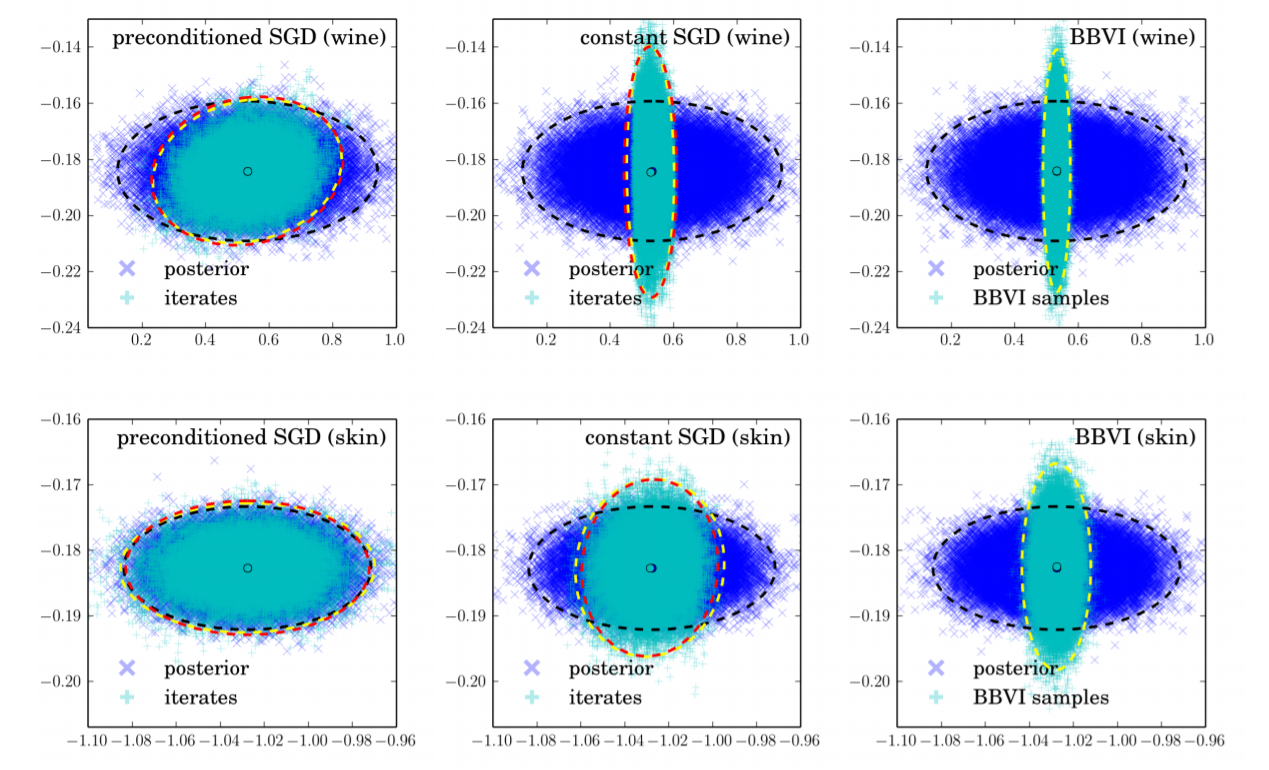
\includegraphics[width=0.75\linewidth]{sgd_inference.png}
    \end{figure} 

    They're projections on the smallest and largest principal component of posterior 
    of two bayesian multivariate regression problems. Blue points come from exact posterior,
    while cyan points come from a inference method.
    
\end{frame}

\begin{frame}
    \frametitle{Quantity result:}

    \begin{figure}[htb]
        \centering
        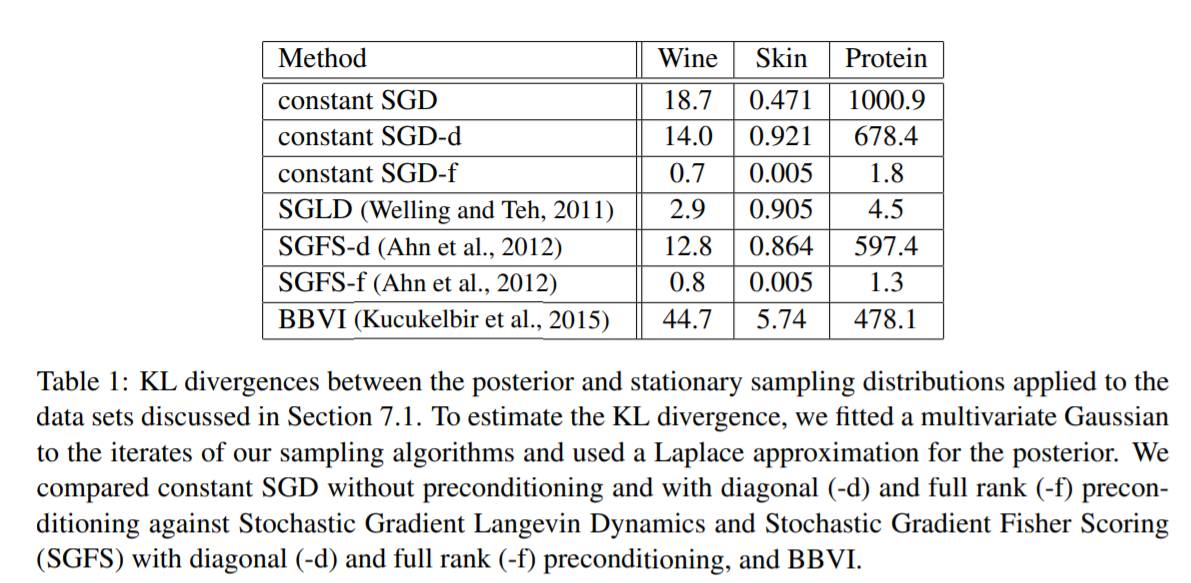
\includegraphics[width=0.75\linewidth]{qc.png}
    \end{figure} 

\end{frame}

\begin{frame}
    \frametitle{Rethink and Criticism: Does those assumption hold?}

    It's hard to image how a posterior distribution of complex enough model is just a normal distribution,
    or can be approximated enough, as assumed by this method. 
    \footnote{Maddox, Wesley, et al. "A simple baseline for bayesian uncertainty in deep learning." arXiv preprint arXiv:1902.02476 (2019).} 
    propose some criticism, such as $C$ is not stationary, observing dynamic of its characteristic, trace: 

    \begin{figure}[htb]
        \centering
        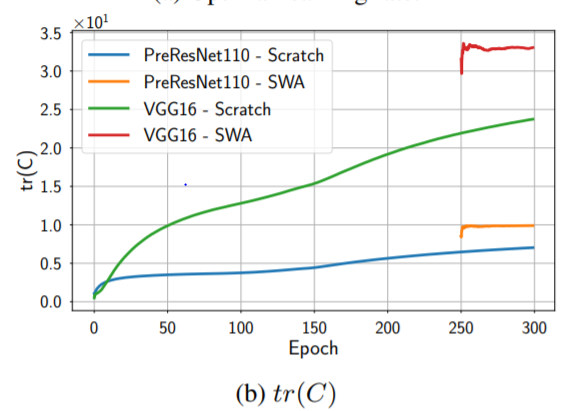
\includegraphics[width=0.5\linewidth]{cri.png}
    \end{figure} 


\end{frame}

\end{document}
